\chapter{Contexto}

Esse projeto tem natureza multidisciplinar, buscando harmonizar a bioquímica do
processo de produção de cervejas com sistemas de controle e automação e
geração e análise de dados estudados na Engenharia Elétrica. Em sua primeira
parte, foi estudado o funcionamento das leveduras e como o ambiente age sobre
seu processo metabólico, enquanto na outra parte, foram estudados sensores,
atuadores e arquitetura de Internet das Coisas para captação, processamento e
disponibilização de informações referente a ação dos microrganismos.

\section{História da Cerveja}

% // TODO: Colocar fontes bibliográficas

% A cerveja pode ser considerada a bebida alcoólica mais antiga do mundo, e atualmente tem uma importância social e econômica muito grande. Durante anos, a sua produção ganhou diversas mudanças, melhorias e adaptações até chegar nas variedades de forma e sabor conhecidas atualmente. 


Segundo \citeonline{Kunze}, a cerveja provavelmente teve origem na revolução agrícola, na qual os humanos começaram a abandonar o nomadismo e se estabeleceram em comunidades que cultivam diversos grãos. Com o armazenamento de cereais, é provável que essa origem tenha sido acidental, com uma fermentação espontânea da cevada. Os mais antigos registros dessa bebida podem ser encontrados na antiga região mesopotâmia, atual Irã, e são datados em 2800 a.C. A sua importância em comunidades antigas do oriente médio era tanta, que em 1760 a.C., foi criada a primeira lei que regulamenta a produção e venda de cerveja. A lei conhecida como Estela de Hamurabi regulamentou a comercialização, fabricação e consumo, estabelecendo uma ração diária de cerveja para os habitantes da região. 


Como o consumo da cerveja era mais seguro do que a água, visto que o processo de fervura ajuda a purificar a bebida, seu consumo em algumas sociedades era visto como uma necessidade básica diária, continua \citeonline{Kunze}. Esse fato ajudou a aumentar a popularidade da bebida na Europa durante a idade média, principalmente nas comunidades Germânicas. Uma das instituições mais importantes para o desenvolvimento dos processos de produção eram os mosteiros dessa região e época. Os monges eram responsáveis pela fabricação da bebida e como eram os únicos que reproduziam os manuscritos, puderam conservar e aperfeiçoar a sua produção, sendo muito influentes até hoje. Eles foram responsáveis por incluir diversas ervas na fabricação, sendo a mais importante delas o lúpulo, utilizado para trazer o amargor da bebida. Uma das leis mais conhecidas e importantes da indústria cervejeira é a da pureza Alemã. Devido a diversas mudanças aplicadas pelos fabricantes e a percepção de uma queda de qualidade, essa lei foi criada no século XIV na região da Bavária (Sul da Alemanha) buscando uma padronização da bebida. A lei instituiu que a cerveja deveria ser fabricada apenas com os seguintes ingredientes: água, malte de cevada e lúpulo. Atualmente, apesar da legalização do uso de qualquer ingrediente na região, muitos cervejeiros ainda seguem essa restrição e ela é um sinônimo de qualidade. 


Ainda segundo \citeonline{Kunze}, uma das mais importantes inovações na fabricação foi a Pasteurização, que permite a preservação do gosto por mais tempo. O processo consiste, basicamente, no aquecimento da bebida a uma determinada temperatura, por determinado tempo, e depois a bebida é resfriada de forma a eliminar os microorganismos ali presentes. O processo foi nomeado pelo seu criador o francês Louis Pasteur que atendendo a solicitação de alguns dos vinicultores e cervejeiros da região que lhe pediram para descobrir como os vinhos e a cervejas azedaram. Durante sua investigação, através do uso de microscópio, ele pôde constatar que a levedura ocasionava este processo e assim criou esse processo de purificação. A partir dele, a indústria cervejeira conseguiu chegar em um novo nível e crescer em escala e alcance, sendo essencial para grandes fábricas atualmente. 


% Atualmente, a indústria de cerveja movimenta milhões de dólares anualmente e uma das divisões que mais cresce são as microcervejarias. No Brasil começaram esses pequenos produtores começaram a surgir na década de 90. Em 2012 as cervejas especiais representavam 8\% do mercado nacional da bebida em 2012 e encerraram 2014 com uma participação de 11\%, segundo o Sindicato Nacional da Indústria da Cerveja, que aponta a existência de 300 microcervejarias no País. A projeção é de que essa cota suba para 20\% em 2020.


\section{Fabricação de Cervejas}

\citeonline{Lewis} apresenta a produção de cerveja como uma atividade que deve equilibrar 
séculos de tradição e arte, desenvolvida por gerações de cervejeiros, e a abordagem científica 
e avanços tecnológicos, de forma que estes possam proporcionar maior entendimento, controle e melhorias 
sobre o processo mas sem abandonar suar raízes históricas e descaracterizá-lo. 
Justamente, as etapas principais do processo ainda seguem a produção tradicional, apesar
da evolução de métodos e técnicas adicionais.

Nesta seção é descrito o processo mais comum de produção de cervejas, considerando os principais
ingredientes: água, malte, lúpulo e levedura. Tradicionalmente, são utilizados grãos maltados de cevada,
mas atualmente podem ser utilizados outros grãos, maltados ou não, como por exemplo: trigo, milho, arroz e aveia.
A partir da descrição de \citeonline{Kunze}, são listadas as principais etapas de produção:


\begin{enumerate}
    \item Maltagem dos grãos: processo de germinação parcial e controlada dos grãos, com a finalidade
de produzir enzimas como a amilase. A germinação é interrompida por um processo de secagem quando atinge o estágio desejado.
A partir desse momento, os grãos passam a ser denominados malte;
    \item Moagem do malte: quebra do malte em pequenos fragmentos para expor as enzimas e componentes internos. É desejável
que parte da casca seja mantida intacta para auxiliar na filtragem após a mostura;
    \item Mostura: o malte moído é misturado em água, e aquecida em temperaturas
que estimulem a ação das enzimas obtidas na maltagem. As enzimas
realizam a quebra de moléculas insolúveis de amido em moléculas menores
de açúcares, que são dissolvidas, formando uma solução denominada mosto;
    \item \textit{Lautering}: o mosto é separado do restante do malte que não foi dissolvido. As
cascas dos grãos auxiliam essa etapa formando um filtro natural, mas também podem ser utilizados filtros;
    \item Fervura: o mosto é fervido, consequentemente: a ação enzimática é
interrompida e a solução é esterilizada. Nessa etapa, lúpulos são adicionados em diferentes
momentos da fervura, fornecendo extratos que conferem amargor e aroma à cerveja;
    \item Fermentação: após o resfriamento do mosto, leveduras são adicionadas e a solução é aerada. 
Os açúcares são consumidos pelo metabolismo das leveduras, gerando etanol e dióxido de carbono;
    \item Maturação: após o consumo dos açúcares, as leveduras passam a reabsorver parte dos
subprodutos gerados durante a fermentação, melhorando a qualidade geral da bebida. Ao final do processo, as leveduras floculam e decantam, podendo ser extraídas e reaproveitadas;
    \item Envase: transferência para o recipiente final. Nessa etapa, também é
realizada a carbonatação da bebida, geralmente por injeção de gás carbônico
ou por meio de uma segunda fermentação, aproveitando-se leveduras ainda presentes na solução.
Industrialmente, é comum a filtragem pré-envase, e a pasteurização pós-
envase.
\end{enumerate}

\subsection{Fermentação e Maturação}

\citeonline{Kunze} posiciona a fermentação como o processo mais importante da produção de cervejas, sendo as etapas
antecedentes responsáveis para garantir as condições necessárias para que as leveduras possam converter os açúcares,
extraídos do malte e quebrados em moléculas menores pelas enzimas, em álcool e gás carbônico. As leveduras consomem 
os açúcares para gerar energia e se reproduzirem, e nesse processo também geram centenas de subprodutos como ésteres, álcoois pesados e compostos sulfúricos que mesmo em pequena quantidade são essenciais para as características organolépticas da cerveja, como
pontuam \citeonline{YeastWhite}.

Leveduras são organismos unicelulares membros do reino fungi. Na produção de cervejas são utilizadas principalmente 
duas espécies: a \textit{Saccharomyces cerevisie} (em cervejas do tipo \textit{Ale}) e a \textit{Saccharomyces pastorianus} (em cervejas do tipo \textit{Lager}). Ao serem inoculadas ao mosto, as leveduras rapidamente absorvem o oxigênio dissolvido para revitalizar sua membrana celular e iniciar a absorção dos açúcares e nutrientes do mosto, descrevem \citeonline{YeastWhite}.
A partir do açúcar absorvido, a levedura pode convertê-lo em energia por meio da respiração aeróbica que ocorre na presença de oxigênio, ou pela respiração anaeróbica que ocorre na ausência de oxigênio ou em solução com alta concentração de glicose (pelo chamado efeito de Crabtree). 
Além da produção energia no formato de moléculas de adenosina trifosfato (ATP), a respiração anaeróbica também produz etanol e gás carbônico, por isso também é denominada de fermentação alcoólica; a equação \ref{eq:fermentacao} ilustra essa reação. A molécula de ATP provém energia para a síntese de proteínas e replicação de DNA, necessários para a multiplicação celular.

\begin{equation}
    Glicose + 2 ADP + 2 Fosfato \longrightarrow 2 Etanol + 2 CO_2 + 2 ATP
    \label{eq:fermentacao}
\end{equation}

A etapa de fermentação e maturação de uma cerveja leva em média entre 7 e 14 dias, desde a inoculação das leveduras até a cerveja estar pronta para envase. Vale notar que podem ser aplicados processos extras na maturação que prolonguem esse tempo.
Para uma fermentação básica, \citeonline{YeastWhite} classificam o processo em 3 fases, que ocorrem com certo grau de sobreposição:
\begin{enumerate}
    \item Fase de retardamento, durante as primeiras quatro a 15 horas após a adição
da levedura no mosto, caracterizada pela climatização das células ao
ambiente e preparação para a próxima fase;
    \item Fase de crescimento exponencial, que dura entre quatro horas e quatro dias,
quando ocorre o consumo dos açúcares e replicação logarítmica das células
de leveduras;
    \item Fase estacionária, em que o crescimento diminui e alguns compostos, como o diacetil, são
absorvidos pelas leveduras, maturando o produto durante três a dez dias.
\end{enumerate}

A variação nas durações das etapas é decorrente tanto da quantidade e saúde das leveduras inoculadas, quanto da temperatura 
durante a fermentação. De acordo com \citeonline{YeastWhite}, tradicionalmente, cervejas do tipo \textit{Ale} são fermentadas a 20°C e cervejas do tipo 
\textit{Lager} a 10°C. Temperaturas inferiores tornam o processo mais lento, e em casos extremos culminar na parada do processo, impedindo a fermentação completa ou que os subprodutos como o diacetil seja absorvido pelas leveduras. temperaturas superiores aceleram a atividade celular, tornando o processo mais rápido, mas também podendo fazer com que as leveduras se multipliquem demais e gerem uma quantidade de subprodutos alta que pode impactar negativamente na qualidade da bebida, gerando sabores indesejados denominados \textit{off-flavors}. 
Justamente por essa razão, o controle de temperatura durante a fermentação é essencial para a obtenção de um produto de 
qualidade com resultados consistentes, principalmente nas primeiras 72 horas do processo, que representam o pico de multiplicação celular, geração de calor decorrente da atividade celular e produção de sub-produtos.

Após a temperatura, \citeonline{YeastWhite} colocam a densidade relativa e pH do mosto como segunda e terceira
variáveis mais importantes para se monitorar durante a fermentação.
A densidade relativa que indica o grau de evolução do processo. Como parte do gás carbônico produzido 
na equação \ref{eq:fermentacao} é dissolvido e capturado pela atmosfera, a densidade do mosto diminui durante a 
fermentação à medida em que os açúcares vão sendo consumidos. A partir disso, é possível: identificar as etapas da 
fermentação pelo gráfico de evolução da densidade relativa ao longo do tempo; estimar a graduação alcoólica a partir dos 
valores inicial e final da densidade relativa; e estipular o grau de atenuação, ou quanto dos açúcares foram consumidos 
pelas leveduras.
Enquanto o pH, que sofre uma leve queda durante o processo, pode ser 
utilizado principalmente como uma amostra das condições iniciais da fermentação, com intuito de se obter reprodutividade do 
processo, e também pode servir como uma variável de diagnóstico de problemas que podem ocorrer como não adaptação das 
leveduras ao mosto e contaminação.

Com caráter ilustrativo, é incluído gráfico com o perfil dessas e outras variáveis durante a fermentação de uma cerveja 
do tipo \textit{Lager} (Figura \ref{fig:variaveis_fermentacao}), retirado de \citeonline{FermentationMunroe}. Na figura, \textit{specific gravity} se refere à
densidade relativa do mosto, e \textit{cells in suspension} à quantidade de células de levedura em suspensão, vale notar que 
ao final do processo, as leveduras floculam e decatam, por isso a queda.

\begin{figure}[H]
    \centering
    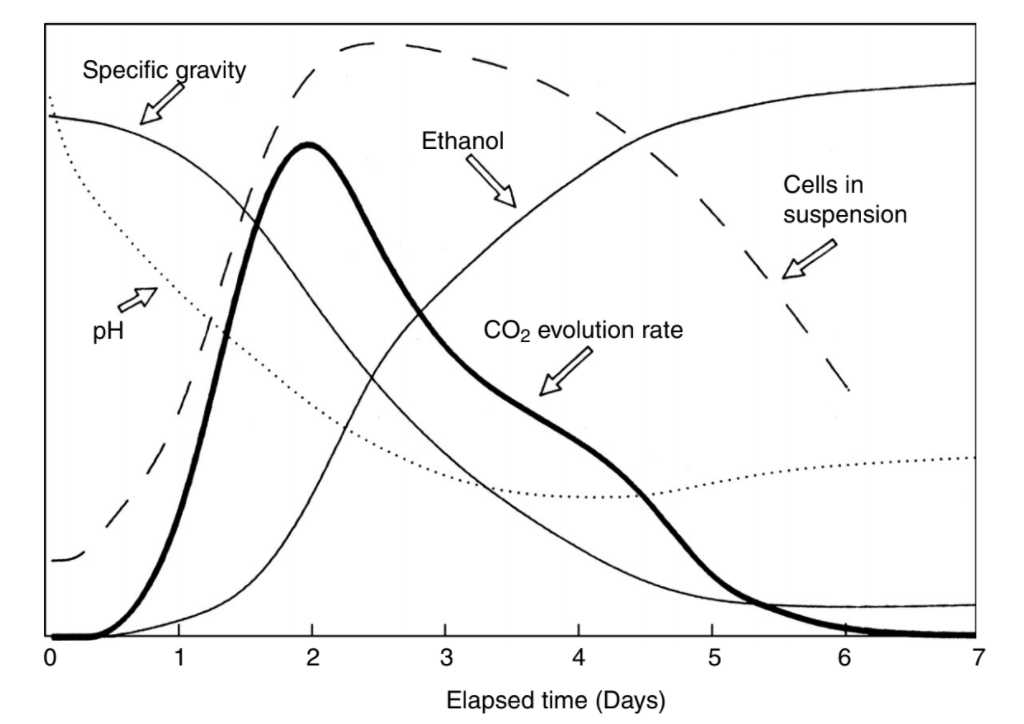
\includegraphics[scale=0.40]{figuras/contexto/variaveis_fermentacao.PNG}
    \captionsource{Gráfico de evolução de variáveis ao longo da fermentação.}{\citeonline{FermentationMunroe}}
    \label{fig:variaveis_fermentacao}
\end{figure}

\section{Análise de Soluções Existentes}


Em produções de grande escala, \citeonline{YeastWhite} afirmam que a maior parte das cervejarias utiliza grandes fermentadores cônicos, que possuem um sistema de resfriamento em seu revestimento, com fluido circulante, para controlar a temperatura durante a fermentação. Para pequenas produções, há uma grande variedade de métodos e equipamentos disponíveis para realizar esse controle, desde sistemas sofisticados que replicam os fermentadores industriais, até métodos manuais.


Empresas como a Grainfather, Ss Brewtech e Birchmann oferecem sistemas de fermentação de primeira linha, com controle de temperatura utilizando a circulação de líquido refrigerante. São modelos relativamente caros, que se assemelham ao equipamento profissional de grande escala. A figura \ref{fig:ssbrewtech} esquematiza um desses produtos, constituído de um compressor para resfriamento do líquido que circula no fermentador por uma serpentina e uma resistência para aquecimento acoplada no fermentador.

\begin{figure}[H]
    \centering
    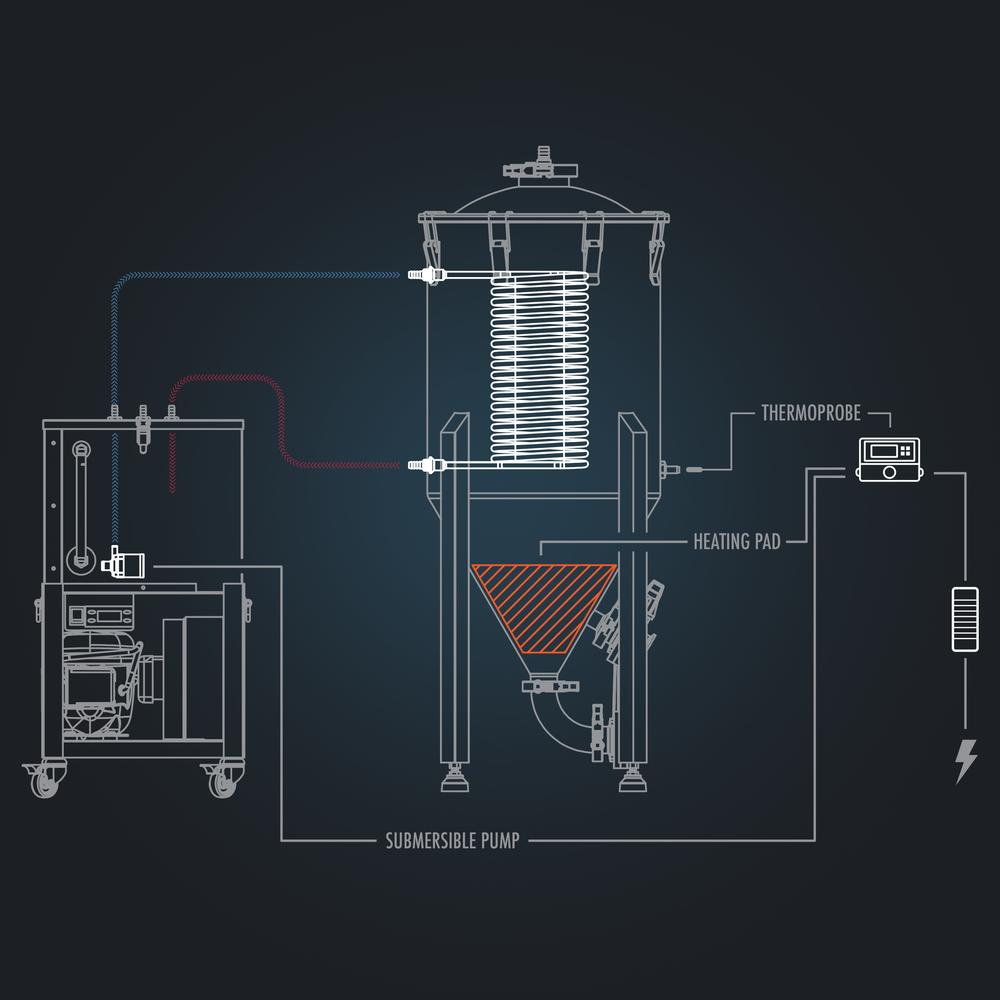
\includegraphics[scale=0.25]{figuras/contexto/glycol_ftss2_1000x.jpg}
    \captionsource{Esquema do equipamento de controle da fermentação FTSs² da Ss Brewtech.}{https://www.ssbrewtech.com/}
    \label{fig:ssbrewtech}
\end{figure}


Na outra extremidade do espectro de soluções, produtores \textit{hobbyistas} que estejam preocupados com o controle de temperatura têm desenvolvido algumas técnicas e equipamentos simples para controle. Um exemplo de técnica comum, é submergir parcialmente o fermentador em um reservatório com água e controlar a temperatura pela adição de gelo nesse reservatório, é um método de baixo custo, mas que exige acompanhamento e esforço constante para se obter um resultado mediano. 


Buscando o controle automatizado, um projeto comum na comunidade de cervejeiros caseiros, é a utilização de geladeiras ou freezers, adaptando-se seu termostato para definição de uma temperatura alvo específica. Esse último método requer um investimento maior na aquisição do refrigerador, mas atinge consegue atingir um bom resultado.
Outra abordagem encontrada é a montagem de um sistema utilizando bomba e serpentina para circulação de um líquido refrigerante. Uma alternativa de menor custo e mais simples em relação ao condensador utilizado na solução já citada, é resfriar o líquido de saída da serpentina em um recipiente com isolamento térmico contendo gelo.


Entre as soluções profissionais e as soluções \textit{hobbyistas} surge uma série de produtos com a finalidade de entregar uma solução pronta e com um custo menor em relação a um sistema completo. Esses produtos tendem a ser comercializados como acessórios que podem ser acoplados a fermentadores de diferentes tamanhos e modelos, sendo mais adaptáveis às necessidades do usuário. As empresas citadas que oferecem sistemas completos também possuem esses \textit{kits} para montagem, além de diversas outras empresas focadas em dispositivos mais simples.


Uma solução bastante interessante é o produto Immersion Pro comercializado pela Brew Jacket (figura \ref{fig:brewjacket}). Ela consiste em controlador que utiliza uma pastilha de Peltier para controle da temperatura (seja resfriamento ou aquecimento) do mosto em fermentação, através de uma haste para troca de calor que fica submersa. É um produto versátil o suficiente para ser instalado nos principais modelos de fermentador e apresenta a capacidade de manter a temperatura com diferença de até 20°C da temperatura ambiente desde que aplicado um isolamento térmico ao fermentador.

\begin{figure}[H]
    \centering
    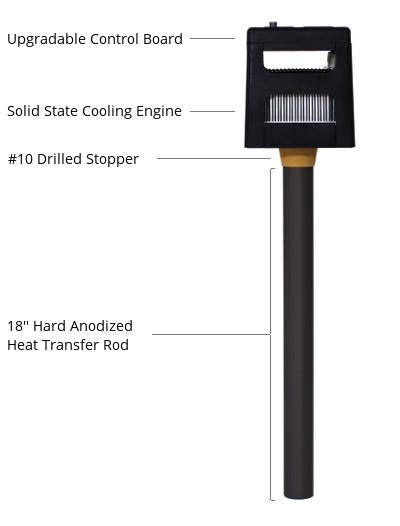
\includegraphics[scale=0.45]{figuras/contexto/brewjacket.jpg}
    \captionsource{Produto Immersion Pro desenvolvido pela Brew Jacket.}{https://brewjacket.com/}
    \label{fig:brewjacket}
\end{figure}

Além das soluções discutidas para controle da temperatura, há uma linha de produtos especializados no monitoramento da temperatura e densidade durante a fermentação e disponibilização online das informações. Dentre as soluções disponíveis, destacam-se pela abordagem na medição da densidade, os produtos Plaato, Beer Bug e Tilt Hydrometer.

A Plaato (figura \ref{fig:plaato}) conseguiu desenvolver uma técnica singular de inferir a densidade do mosto pelo volume de \(CO_2\) que é expelido durante a fermentação. O produto na forma de um \textit{airlock} é conectado ao fermentador vedado e envia os dados de densidade e temperatura coletados via conexão \textit{Wi-Fi}, que podem ser acompanhados em computadores ou dispositivos móveis. Também com disponibilização dos dados de temperatura e densidade online, o Tilt Hydrometer (figura \ref{fig:tilt}) é um pequeno dispositivo cilíndrico que fica imerso no fermentador e infere a densidade pelo ângulo de inclinação de flutuação, enquanto que o Beer Bug (figura \ref{fig:beerbug}) é instalado como um \textit{airlock} e infere a densidade medindo a força de empuxo sofrida por uma carga submersa no mosto e conectado ao dispositivo por um fio.

Analisando as soluções existente, este projeto se posiciona com o objetivo de desenvolver um protótipo que reúna o controle de temperatura com o monitoramento online das variáveis relevantes. Além disso, que possa ser desenvolvido em um produto razoavelmente versátil para ser instalado em fermentadores comuns.

\begin{figure}[h]
    \centering
    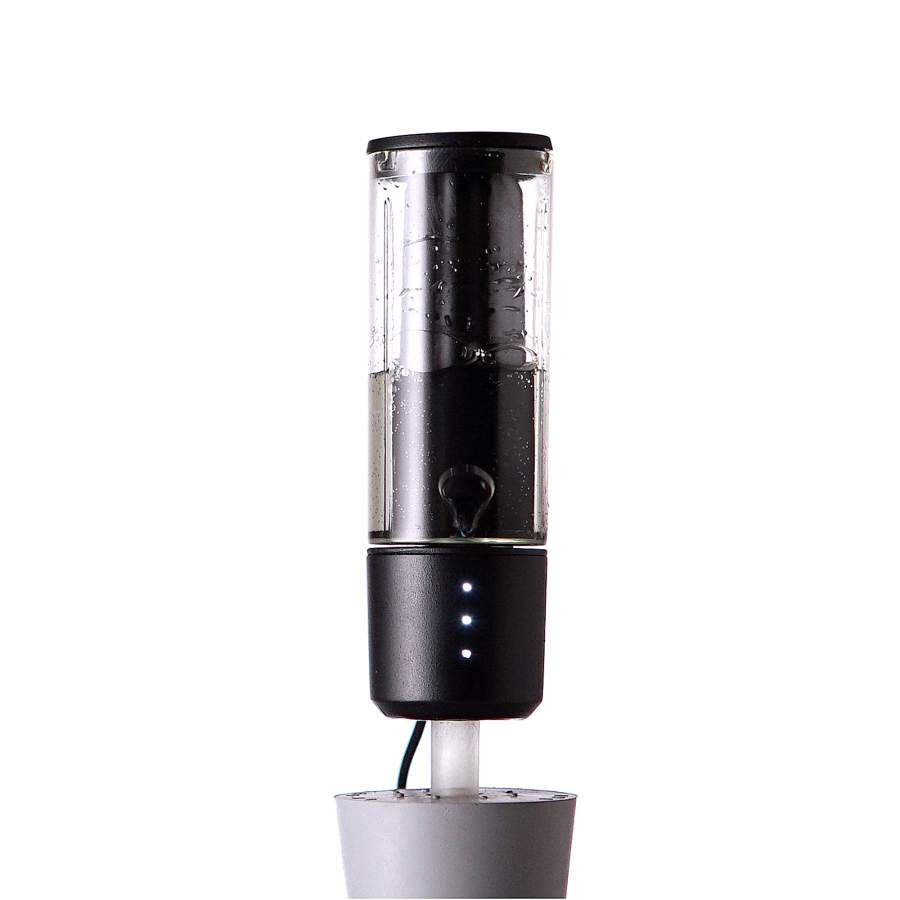
\includegraphics[scale=0.25]{figuras/contexto/plaato.jpg}
    \captionsource{Solução Plaato.}{https://plaato.io/}
    \label{fig:plaato}
\end{figure}


\begin{figure}[h]
    \centering
    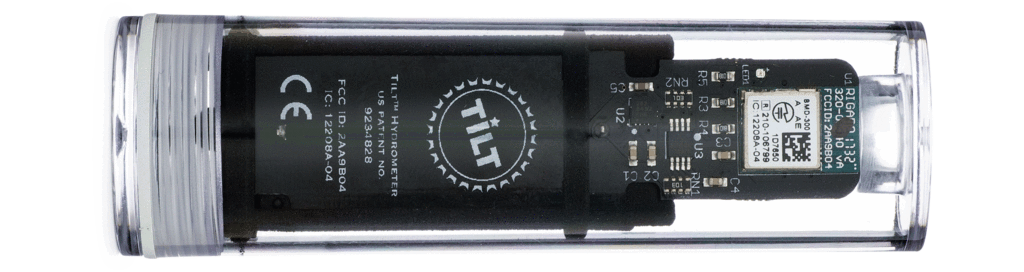
\includegraphics[scale=0.45]{figuras/contexto/tilt.png}
    \captionsource{Solução Tilt Hydrometer.}{https://tilthydrometer.com/}
    \label{fig:tilt}
\end{figure}

\begin{figure}[h]
    \centering
    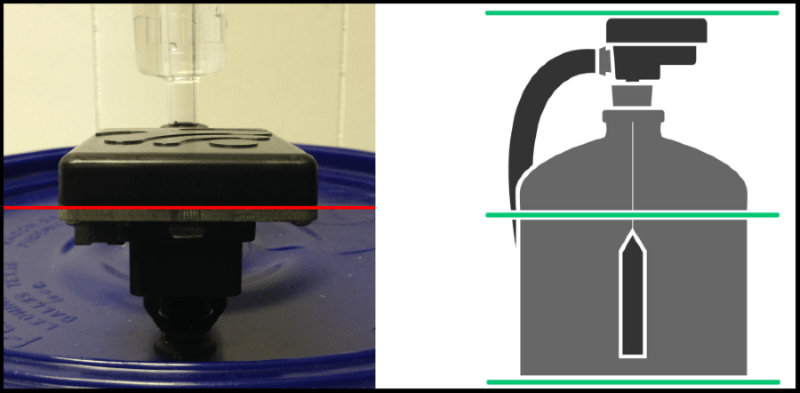
\includegraphics[scale=0.35]{figuras/contexto/beerbug.png}
    \captionsource{Solução Beer Bug.}{https://straighttothepint.com/}
    \label{fig:beerbug}
\end{figure}

